\documentclass{article}
\usepackage{graphicx}
%permite ecribir acentos directamente
\usepackage[utf8]{inputenc}
% Esto es para que el LÁTEX sepa que el texto está en español, se agrega el ingles para el paquete de gráfico de circuitos:
\usepackage[spanish]{babel}
\usepackage{geometry}
 \geometry{a4paper,total={170mm,257mm},left=15mm,right=15mm,top=20mm,}
\usepackage{hyperref} 
\usepackage{amsmath, amsfonts}
\usepackage{enumitem}
\usepackage{xcolor}
\usepackage{textcomp}
\usepackage{fancyhdr}

\pagestyle{fancy}
\fancyhf{}
\lhead{Electronica de Potencia}
\rhead{TP1 : Control de ángulo de conducción de un SCR}
\rfoot{Page \thepage}

\begin{document}
\begin{titlepage}
 \centering
	
\includegraphics[scale=0.80]{imagenes/LOGO.jpg} \par
 	\vspace{1cm}
 	{\scshape\LARGE Universidad Tecnológica Nacional \par}
 	{\scshape\large Facultad Regional de Córdoba \par}
 	\vspace{1cm}
	{\bfseries \Large Trabajo Práctico De Laboratorio $N^{\circ} 2$\par}
	{\bfseries \Large Control de ángulo de conducción de un SCR \par}
 	\vspace{1.5cm}

	\begin{tabular}{ll}
		Alassia, Francisco	&	60861	\\
		Amaya, Matías		&	68284	\\
		Lamas, Matías 		&	65536 	\\
		Navarro, Facundo 	&	63809 	\\
		Veron, Misael	 	&	62628
	\end{tabular}
	
	\vspace{1cm}
	Curso: 5r2 \\
	Grupo $N^{\circ} 11$
 	\vfill
	{\bfseries \Large Electrónica de Potencia \par}

	\vspace{1.5cm}
	Docentes: \par
	Ing. Oros \par
	Ing. Rabinovich \par

 	\vfill
	{\large \today\par}
\end{titlepage}

%##################################### INDICE  #####################################################

\tableofcontents
\clearpage

%##################################### INDICE  #####################################################

\section{Introducción}
Diseñar y construir un circuito para el control del ángulo de conducción de un SCR mediante el método escalón-rampa coseno. La tensión en la carga debe ser controlada por una señal de reverencia $V_{reff}$ , que variará entre 0 y 10 $V$.


\subsection{Funcionamiento}
La figura \textcolor{blue}{\ref{fig:fig1}} al circuito de control del ángulo de conducción de onda completa de un SCR con disparo por UJT. El circuito del método escalón-rampa coseno de la figura \textcolor{blue}{\ref{fig:fig2}}  , deriva del circuito anterior con el agregado de algunas variantes que permite mayor linealidad entre la tensión de referencia y la tensión en la carga.

\begin{figure}[h]
 \begin{center}
	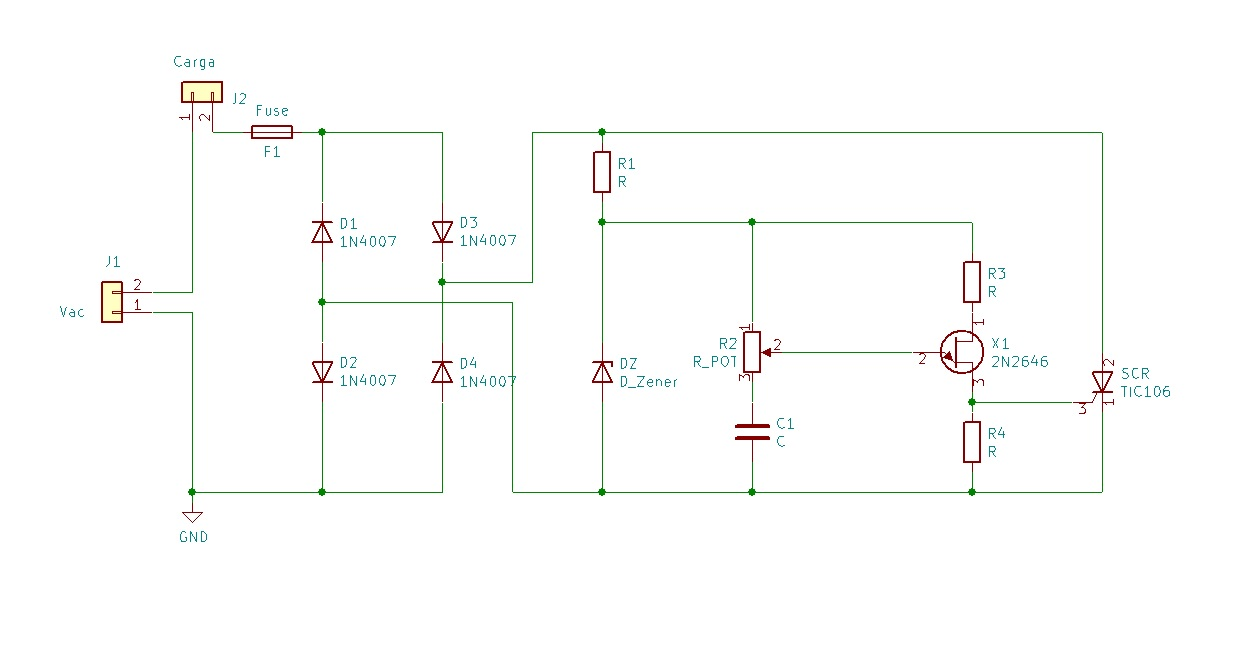
\includegraphics[scale=0.7]{imagenes/fig1.jpg} 
	\caption{Control de ángulo de conducción de un SCR por un UJT}\label{fig:fig1}
 \end{center}
\end{figure}

Cuando $V_C1$ se iguala a la tensión $V_P$ (disparo del unijuntura), éste se dispara y genera un impulso de corriente entre sus bases que, a su vez produce el disparo del SCR.

\begin{figure}[h]
 \begin{center}
	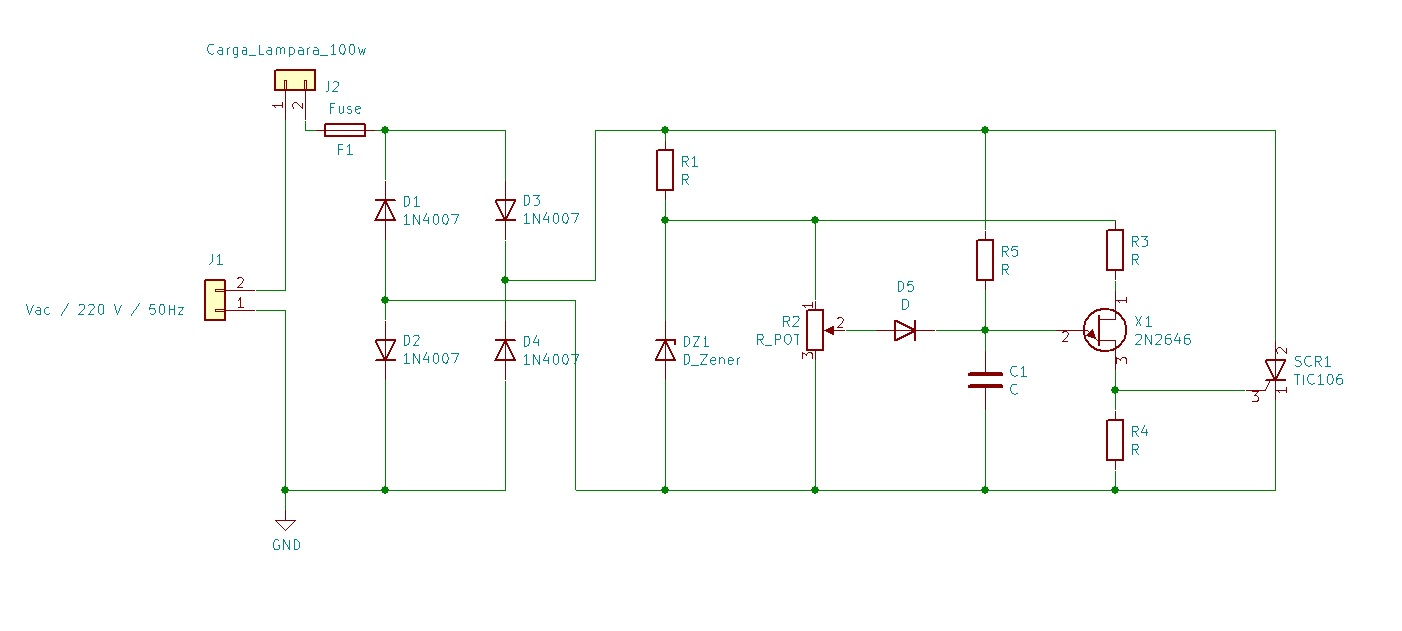
\includegraphics[scale=0.6]{imagenes/fig2.jpg} 
	\caption{Circuito escalón-rampa coseno}\label{fig:fig2}
 \end{center}
\end{figure}

El método escalón-rampa consiste en cargar el capacitor con un escalón inicial de amplitud variable (malla $R_2$ - $D_5$ - $C_1$) y luego con una rampa de pendiente fija (rama $R_5$ - $C_1$). El capacitor se carga inicialmente a través de la resistencia del potenciómetro $R_2$ y del diodo $D_5$. Una vez cargado con el escalón inicial, el diodo deja de conducir y el capacitor pasa a cargarse con la tensión rectificada de la línea a través de $R_5$ hasta que $V_{C1}$ se iguala a la tensión $V_P$ produciendo el disparo del UJT.

La malla $R_2$ - $D_5$ - $C_1$ se define como constante de tiempo $\tau_1$ y la rama $R_5$ - $C_1$ como $\tau_2$, siendo el valor de la misma mucho mayor que $\tau_1$ de forma que la tensión en el capacitor forme una rampa. El valor de esta constante $\tau_2$ debe satisfacer el caso de que el escalón inicial sea nulo (el potenciómetro en su extremo inferior), para que la tensión en el capacitor llegue a la tensión de disparo ($10 V$) en un semiciclo de la tensión de entrada.

Si se modifica la rampa de forma que su crecimiento no sea lineal, sino cosenoidal, se logra que la tensión de referencia $V_C$ (tensión instantánea en el capacitor) y la tensión aplicada en la carga $V_L$, sea prácticamente lineal.

El puente de diodos $D_1$-$D_4$, son los encargados de rectificar la tensión de línea para el correcto funcionamiento del SCR. $R_1$ limita la corriente que circuila por el diodo zener.
%
\section{Desarrollo}
Para el diseño, los dispositivos elegidos son los siguientes:
\begin{itemize}\itemsep0em \itemindent=2em
	\item[•]{\makebox[0.9cm]{SCR\hfill}: TIC 106}
	\item[•]{\makebox[0.9cm]{UJT\hfill}: 2N2646}
	\item[•]{\makebox[0.9cm]{Zener\hfill}: 1N4745}
	\item[•]{\makebox[0.9cm]{Diodo\hfill}: 1N4007}
\end{itemize}
%
\subsection{Cálculos}
Por consigna, debe efectuarse para una carga resistiva de $220\;V_{RMS}$ y $1\;kW$, entonces
\begin{align*}
	I_L &= \frac{P_L}{V_L} \\
	I_L	&= \frac{1000\;W}{220\;V_{RMS}} \\
	I_L	&= 4,54 \; A_{RMS}
\end{align*}

De la hoja de datos del SCR, se tiene:
%
\begin{itemize}\itemsep0em \itemindent=2em
	\item[•]{\makebox[1cm]{$V_{DRM}$\hfill}= $400 \; V$}
	\item[•]{\makebox[1cm]{$I_T$\hfill}= $5 \; A$ a 80\textdegree{C}}
	\item[•]{\makebox[1cm]{$I_{GT}$\hfill}= $200 \; \mu A$}
	\item[•]{\makebox[1cm]{$V_{GT}$\hfill}= $1,2 \; V$}
\end{itemize}
Para garantizar que el disparo se encuentre siempre dentro de la zona de disparo seguro, se establece:
\begin{align*}
	I_G &= 5 * I_{GT} \\
	I_G	&= 1 \; mA
\end{align*}
%
De la hoja de datos del UJT, se tiene:
\begin{itemize}\itemsep0em \itemindent=2em
	\item[•]{\makebox[1.8cm]{$\eta$\hfill}= $0,75$}
	\item[•]{\makebox[1.8cm]{$R_{BB(off)}$\hfill}= $7 \; k\Omega$}
	\item[•]{\makebox[1.8cm]{$R_{BB(on)}$\hfill}= $600 \; k\Omega$}
\end{itemize}
%
Los valores de las resistencias de las bases son, por la relación:
\begin{align*}
	\eta &= \frac{R_{BB1}}{R_{BB(off)}} \\
	\eta &= \frac{R_{BB1}}{R_{BB1} + R_{BB2}}\\
\end{align*}
entonces, 
\[R_{BB1} = 5250 \; \Omega \; ; \; R_{BB2} = 1750 \; \Omega \]
\clearpage
%
\subsubsection{Cálculos de $R_3$, $R_4$ y $V_Z$}
En la figura \textcolor{blue}{\ref{fig:fig3}} se muestra el circuito equivalente con el agregado de las resistencias que procederemos a calcular como así también la curva característica del UJT.
%
\begin{figure}[h]
 \begin{center}
	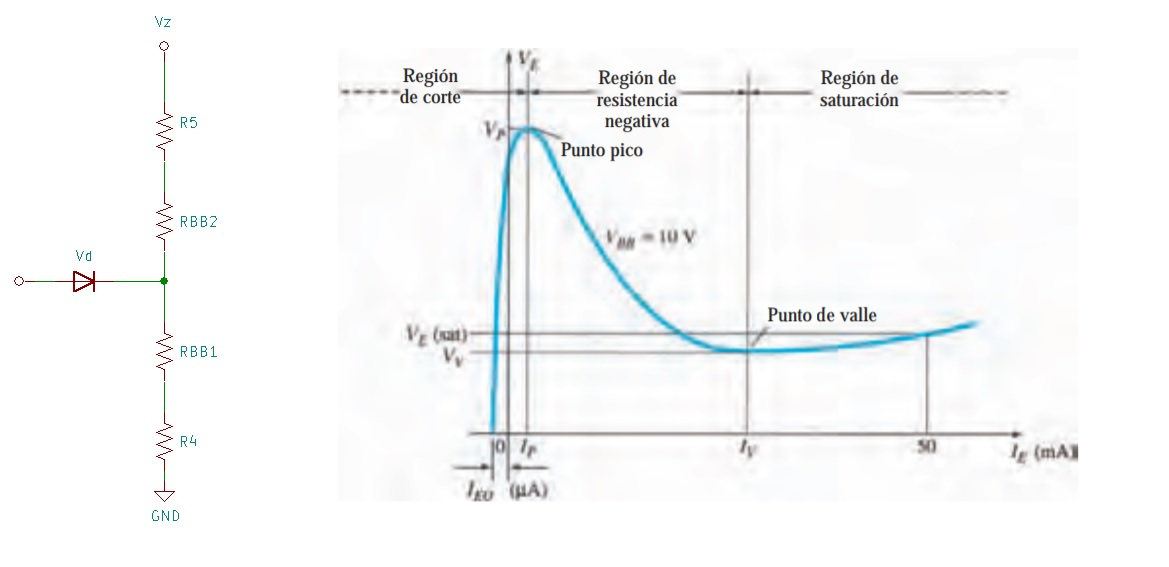
\includegraphics[width=\textwidth]{imagenes/fig3.jpg} 
	\caption{Circuito equivalente y curva característica}\label{fig:fig3}
 \end{center}
\end{figure}
%
La corriente que debe circular entre la base 2 y la base 1 debe ser mucho mayor que la requerida por el SCR, 
\[ I_{B2B1(on)} = 15 \; I_G \]
La tensión en $R_4$, debe ser la necesaria para el disparo del SCR y la corriente en la resistencia será la diferencia entre $I_{B2B1(on)}$ e $I_G$
\begin{align*}
V_{GT} &= R_4 * (I_{B2B1(on) - I_G}) \\
V_{GT} &\approx 82 \; \Omega  
\end{align*}

Por otro lado, $V_P$ por consigna debe ser 10 V, entonces
\[V_{E(off)} < 10 \; V \; ; \; V_{E(on)} > 10 \; V\]

Cuando el UJT no está disparado, la tensión entre $R_{BB1}$ y $R_4$ debe ser
\begin{align*}
V_{E(off)} &= V_D + \eta V_{B2B1} + V_{R4} \\
V_{E(off)} &= V_D + V_{B1R4}\\
\end{align*}

quedando

\[ V_{B1RA} = 9,5 \; V \]

y la corriente 
\[ I_{B2B1(off)} = \frac{V_{B1RA}}{R_{BB1} + R_4} = 1,782 \; mA \]

La tensión en la base 2 es
\[ V_{B2} = I_{B2B1(off)} (R_{BB} + R_4) = 12.62 \; V \]
y en $R_3$

\begin{equation}
I_{B2B1(off)} * R_3 = V_Z - V_{B2}  \label{eq:uno}
\end{equation}

Por otro lado, cuando el UJT es disparado la resistencia $R_{BB}$ desciende a $600 \; \Omega$ entonces
\begin{align}
V_Z &= V_{R3} + V_{B2B1} + V_{R4} \nonumber \\
V_Z &= I_{B2B1(on)} (R_3 + R_{BB} + R_4) \label{eq:dos}
\end{align}
%
De lo anterior, se puede formar un sistema de ecuaciones entre las ecuaciones \ref{eq:uno} y \ref{eq:dos}, se obtiene
\[ R_3 = 180 \; \Omega \]
\[ V_Z \approx 13 \; V\]
%
\subsubsection{Cálculo de $R_5$, $R_1$ y $C_1$}
Como se definió al principio $\tau_1$ corresponde a $R_2C_1$ y $\tau_2$ a $R_5C_1$. Se forzará a que el capacitor se encuentre completamente cargado a su valor final luego de un tiempo 20 veces menor al semiciclo de la tensión de red
\[ \tau_1 = \frac{10 \; ms}{20} = 500 \mu s \]
Si se elige $C_1 \; = \; 100nF$ entonces
\[ R_2 = \frac{500 \; \mu s}{100 \; nF} = 5 \; k \Omega \]
Suponiendo el caso en el que la tensión del escalón es de $0 \; V$, el capacitor deberá cargarse al valor de $10 \; V$ a través de $R_5$ en un tiempo de $10 \; ms$. Suponiendo una señal cuadrada en lugar de una senoidal y la amplitud aplicada a la resistencia $R_1$ de $V_{AC_P} = 311 \; V $, se tiene 
%
\[ C_1R_5 = \frac{V_{ACpico}}{V_{C max}} * 10 \; ms \]
quedando
\[ R_5 = 3,1 \; M \Omega \]

\subsection{Circuito Final}
Se termina presentando el esquemático final con el agregado de los valores de los componentes, además se aclara que se agrega dos potenciómetros de tipo trimmer con el fin de calibrar el circuito ante variaciones de los valores de los componentes.
\begin{figure}[h]
 \begin{center}
	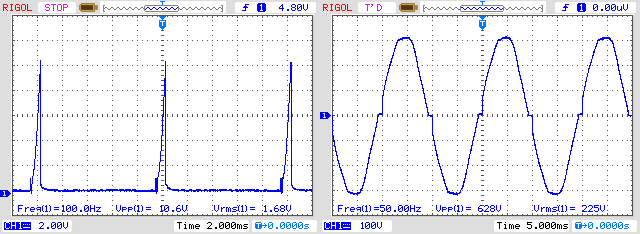
\includegraphics[width=\textwidth]{imagenes/fig5.jpg} 
	\caption{Circuito final}\label{fig:fig5}
 \end{center}
\end{figure}

\clearpage

\subsection{Mediciones y experimentación}
\begin{center}
\begin{tabular}{| c | c | c |}
\hline
$V_{REF}$ (Capacitor) & $V_{RMS}$ (Carga) & Angulo [grados] \\
\hline
&&\\
\hline 
&&\\
\hline 
&&\\
\hline 
&&\\
\hline 
&&\\
\hline 
&&\\
\hline 
&&\\
\hline 
&&\\
\hline 
&&\\
\hline 
&&\\
\hline 
&&\\
\hline 
&&\\
\hline 
&&\\
\hline 
&&\\
\hline 
&&\\
\hline 
&&\\
\hline 
&&\\
\hline 
&&\\
\hline 
&&\\
\hline 
&&\\
\hline 
&&\\
\hline 
&&\\
\hline 
&&\\
\hline 
&&\\
\hline 
\end{tabular}
\end{center}

\clearpage
\section{Conclusión}
El método escalón-rampa coseno presenta las siguientes ventajas y desventajas:

\begin{itemize}
\item[•] Ventajas
	\begin{itemize}
		\item[*] Se puede emplear para un control preciso de la intensidad lumínica de una lámpara, la temperatura de un soldador u otros dispositivos alimentados con la tensión de la red.
		\item[*] Requiere de dispositivos de baja potencia.
		\item[*] Circuito de bajo costo y fácil implementación.
	\end{itemize}
\item[•] Desventajas
	\begin{itemize}
		\item[*] Para lograr una buena linealidad requiere que los componentes utilizados sean lo más exactos posibles.
		\item[*] El valor de la resistencia de la carga debe ser menor que la resistencia total del circuito de control.
	\end{itemize}
\end{itemize}

Por requisito, la tension máxima de referencia debe ser de $10 \; V$ para ello se coloca una resistencia en serie ubicada en el extremo superior del potenciómentro, sabiendo que:
\begin{itemize}\itemsep0em \itemindent=2em
	\item[•]{\makebox[1,7cm]{$I_{R1}$\hfill}= $30 \; mA$}
	\item[•]{\makebox[1,7cm]{$I_Z$\hfill}= $20 \; mAC$}
	\item[•]{\makebox[1,7cm]{$I_{B2B1(off)}$\hfill}= $1,8 \;  mA$}
\end{itemize}

La corriente que circula por la rama del potenciómentro cuanto el UJT se encuentra apagado es:
\begin{align*}
I_{pot} &= I_{R1} - I_Z - I_{B2B1(off)} \\
I_{pot} &= 8,2 \; mA
\end{align*}
quedando finalmente
\begin{align*}
R_{sup} &= \frac{5,3 \; V}{8,2 \; mA} \\
R_{sup} &\approx 680 \; \Omega
\end{align*}

Debido a la no exactitud del valor, tanto del capacitor como el de las resistencias, el circuito presenta una alinealidad entre el giro del potenciómetro en la zona mínima y el ángulo de conducción. Para poder mejorar este defecto se coloca una resistencia en serie ubicada en el extremo inferior para que la tensión del escalón arranque desde un valor mínimo.
\begin{align*}
R_{inf} &= \frac{4,8 \; V}{8,2 \; mA} \\
R_{inf} &\approx 560 \; \Omega
\end{align*}

\end{document}